\documentclass[hyperref, a4paper]{article}

\usepackage{geometry}
\usepackage{float}
\usepackage{titling}
\usepackage{titlesec}
% No longer needed, since we will use enumitem package
% \usepackage{paralist}
\usepackage{enumitem}
\usepackage{footnote}
\usepackage{enumerate}
\usepackage{amsmath, amssymb, amsthm}
\usepackage{mathtools}
\usepackage{bbm}
\usepackage{cite}
\usepackage{graphicx}
\usepackage{subcaption}
\usepackage{physics}
\usepackage{tensor}
\usepackage{siunitx}
\usepackage{booktabs}
\usepackage[version=4]{mhchem}
\usepackage{tikz}
\usepackage{xcolor}
\usepackage{listings}
\usepackage{autobreak}
\usepackage[ruled, vlined, linesnumbered]{algorithm2e}
\usepackage{xr-hyper}
\usepackage[colorlinks,unicode]{hyperref} % , linkcolor=black, anchorcolor=black, citecolor=black, urlcolor=black, filecolor=black
\usepackage{prettyref}

% Page style
\geometry{left=3.18cm,right=3.18cm,top=2.54cm,bottom=2.54cm}
\titlespacing{\paragraph}{0pt}{1pt}{10pt}[20pt]
\setlength{\droptitle}{-5em}
\preauthor{\vspace{-10pt}\begin{center}}
\postauthor{\par\end{center}}

% More compact lists 
\setlist[itemize]{itemindent=17pt, leftmargin=1pt}

% Math operators
\DeclareMathOperator{\timeorder}{\mathcal{T}}
\DeclareMathOperator{\diag}{diag}
\DeclareMathOperator{\legpoly}{P}
\DeclareMathOperator{\primevalue}{P}
\DeclareMathOperator{\sgn}{sgn}
\newcommand*{\ii}{\mathrm{i}}
\newcommand*{\ee}{\mathrm{e}}
\newcommand*{\const}{\mathrm{const}}
\newcommand*{\suchthat}{\quad \text{s.t.} \quad}
\newcommand*{\argmin}{\arg\min}
\newcommand*{\argmax}{\arg\max}
\newcommand*{\normalorder}[1]{: #1 :}
\newcommand*{\pair}[1]{\langle #1 \rangle}
\newcommand*{\fd}[1]{\mathcal{D} #1}
\DeclareMathOperator{\bigO}{\mathcal{O}}
\DeclareMathOperator{\object}{Ob}
\DeclareMathOperator{\morphism}{Hom}

% TikZ setting
\usetikzlibrary{arrows,shapes,positioning}
\usetikzlibrary{arrows.meta}
\usetikzlibrary{decorations.markings}
\tikzstyle arrowstyle=[scale=1]
\tikzstyle directed=[postaction={decorate,decoration={markings,
    mark=at position .5 with {\arrow[arrowstyle]{stealth}}}}]
\tikzstyle ray=[directed, thick]
\tikzstyle dot=[anchor=base,fill,circle,inner sep=1pt]

% Algorithm setting
% Julia-style code
\SetKwIF{If}{ElseIf}{Else}{if}{}{elseif}{else}{end}
\SetKwFor{For}{for}{}{end}
\SetKwFor{While}{while}{}{end}
\SetKwProg{Function}{function}{}{end}
\SetArgSty{textnormal}

\newcommand*{\concept}[1]{{\textbf{#1}}}

\newrefformat{fig}{Figure~\ref{#1}}

% Embedded codes
\lstset{basicstyle=\ttfamily,
  showstringspaces=false,
  commentstyle=\color{gray},
  keywordstyle=\color{blue}
}

\title{Quantum Optics, Homework 2}
\author{Jinyuan Wu}

\begin{document}

\maketitle

This document has been revised to include contents on the discussion session held on November 7, 2021.

\begin{figure}
    \centering
    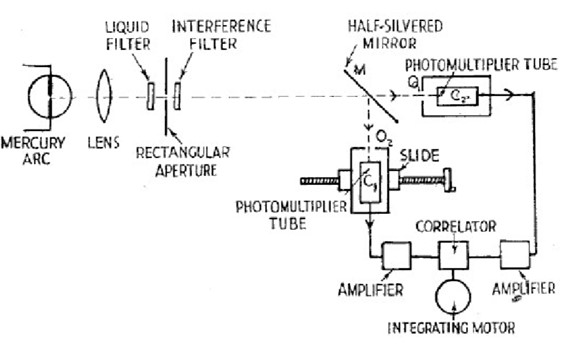
\includegraphics[width=0.65\textwidth]{hbt-lab.png}
    \caption{HBT effect in laboratory}
    \label{fig:hbt-lab}
\end{figure}

\begin{figure}
    \centering
    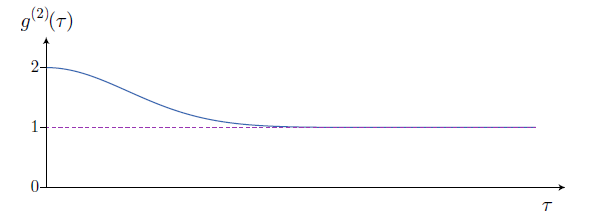
\includegraphics[width=0.6\textwidth]{thermal-state-g2.PNG}
    \caption{Second order coherence with a thermal light source in Gaussian distribution (figure taken from \cite{optical-note-steck}, Section~2.6.1).
    The maximum of $g^{(2)}$ is 2, which is a result of the optical field obeying a Gaussian distribution, where the Wick theorem holds so $\expval{E^*_1 E^*_2 E_3 E_4} = \expval{E^*_1 E_3} \expval{E^*_2 E_4} + \expval{E^*_1 E_4} \expval{E^*_2 E_3}$, and hence $\expval*{I^2} = 2 \expval{I}^2$.
    Experimentally, the maximum may not be achieved due to fluctuations that destroy the correlation.}
    \label{fig:thermal-hbt}
\end{figure}

\paragraph{Details in the HBT experiment} \prettyref{fig:hbt-lab} shows an experimental validation of the HBT effect. 
(a) Describe the expected phenomenon the experiment. Compare the expected phenomenon with the original HBT effect in astronomical observation.
(b) Explain the phenomenon within classical electrodynamics.
(c) Point out why the classical explanation is not enough. Construct a simplified version of the experiment and explain it with quantum optics.

\paragraph{Solution} \begin{itemize}
    \item[(a)] The integrating motor gives the averaged intensity correlation function, i.e.
    \begin{equation}
        \expval*{I_1 I_2} \coloneqq \lim_{T \to \infty} \frac{1}{T} \int_0^T \dd{t} I_1(t) I_2(t). 
    \end{equation} 
    The expected results include that
    \begin{equation}
        \expval*{I_1 I_2} - \expval{I_1} \expval{I_2} \neq 0, \quad g^{(2)} > 1,
    \end{equation} 
    and that the intensity fluctuation correlation function 
    \begin{equation}
        \expval{\Delta I_1 \Delta I_2} = \expval*{I_1 I_2} - \expval{I_1} \expval{I_2}
    \end{equation}
    reaches its peak when the optical path difference of the two beams is zero, 
    and then drops away as the separation between the two beams increases. 
    If the light source is laser, the relation between $g^{(2)}$ and the optical path difference is in the form 
    of $1 + \cos(k \Delta r)$, while if the light source is thermal - as is the case of a mercury arc - 
    the relation between $g^{(2)}$ and the optical path separation is something like \prettyref{fig:thermal-hbt}.

    The experiment shown in \prettyref{fig:hbt-lab} is \emph{essentially the same} with the astronomical HBT experiment.
    Note that the movable detector is moved \emph{horizontally} so that the input light must have several components with different wave vector directions, 
    and the beam from the mercury light is \emph{never} collimated.
    The input light in \prettyref{fig:hbt-lab} is indeed \emph{multi-mode}, where the wave vectors can take different directions.
    This is indeed the same with the case in astronomical HBT experiment.
    The ``star'' in \prettyref{fig:hbt-lab} is the aperture.

    Note that the device shown in \prettyref{fig:hbt-lab} can be adjusted to measure the second order \emph{temporal} correlation 
    rather than the second order \emph{spacial} correlation, as long as the movable detector is moved vertically instead of horizontally.

    \item[(b)] The correlation function involved in the second order coherence is  
    \begin{equation}
        \expval{I_1 I_2} = \expval*{ I_1(t) I_2(t) } .
    \end{equation}
    
    With a thermal light source, when the two detectors are separated far enough, $E_1$ and $E_2$ are not correlated, and we have 
    \[
        g^{(2)} = \frac{\expval{I_1 I_2}}{\expval{I_1} \expval{I_2}} \approx \frac{\expval{I_1} \expval{I_2}}{\expval{I_1} \expval{I_2}} = 1.
    \]
    When the two detectors are almost observing the same $\vb*{E}$ components, however, we have 
    \[
        \expval{(I_1(t) - \expval*{I_1}) (I_2(t) - \expval*{I_2})} = \expval{(I_1(t) - \expval*{I_1})^2}> 0,
    \]
    and subsequently
    \[
        \expval*{I_1 I_2} - \expval*{I_1} \expval*{I_2} > 0, 
    \]
    so $g^{(2)} > 1$.
    So we have something like \prettyref{fig:thermal-hbt}.

    \item[(c)] When the classical picture of the optical field fails, the classical explanation fails as well.
    For example, when the light source creates a sequence of single-photon pulses, what will be observed is \emph{photon antibunching} where $g^{(2)} = 0$ instead of bunching, because one photon cannot appear at two sites.
\end{itemize}

\paragraph{Discussion} \begin{itemize}
    \item[(a)] We did not calculate the correlation length of $g^{(2)}$ because it cannot be easily done for an arbitrary state of the optical field.
    
    For a original light beam from a star, the correlation length given by $g^{(2)}$ is definitely affected by the 
    temperature of the optical field generated by the star when the HBT experiment is used astronomically. 
    The temperature determines the power distribution on different frequencies and the photon numbers on each mode.
    To relief ourselves from the burden to calculate $g^{(2)}$ under such a terrible state, when the HBT experiment is done, 
    we usually \emph{filter} the light from the star to be measured to obtain a single-frequency optical field.

    The correlation length obtained from the second order coherence between two plane waves with a slightly different wave vector 
    is $\lambda / \theta$, where the angle $\theta$ is the angle between the wave vectors. 
    The second order coherence between two plane waves is periodic, but since each point on the surface of the star in question 
    radiates plane waves, after adding all components, we again get something like \prettyref{fig:thermal-hbt}.
    If we know the geometry of the surface of the star, the correlation length in \prettyref{fig:thermal-hbt} can be obtained.
    The light after the monochromatic filter is still thermal, but the thermal nature of the light can be seen as adding a random 
    phase to each plane wave component, which is not involved in the second-order coherence, the temperature of the optical field
    \emph{does not} affect the correlation length.
\end{itemize}

\paragraph{}

\paragraph{Conditional generation of single photon pulses} Many research and applications in quantum optics needs single photon pulses, that is, a wave packet of light that contains exactly one single photon. Such a single photon pulse can be generated in two ways: The deterministic approach via single atom emission, and the so-called heralded approach. This problem discusses a simplified version of the later.
Consider a bi-photon generation process described by the Hamiltonian  
\begin{equation}
    H=\beta a_{k}^\dagger b_{k^{\prime}}^\dagger+ \text{h.c.}.
\end{equation}
Here $a_{k}^\dagger, b_{k^{\prime}}^\dagger$ are creation operators of photons into the $k, k'$ propagation modes respectively. Such process can be realized for example in a frequency down conversion experiment, where a single photon is ``split'' into two in a nonlinear optical crystal, or a 4-wave mixing experiment where two incoming photons are converted into two output photons in an atomic gas.
(a) Consider initially light is in vacuum state $|\psi(0)\rangle=|V\rangle$. Consider that the bi-photon generation process is switched on for time $\tau$ and then off, with $\xi=\beta \tau \ll 1$. Integrate the Schrodinger equation to obtain $|\psi(\tau)\rangle$, that is, the photon state after the interaction. (b) Consider a photon detector positioned $L$ meters away from the bi-photon generation device along the $k'$ propagation pathway. The time interval that the detector can detect a $b_{k'}$ photon is $[L / c, L / c+\tau]$ (we ignore any change of light speed within the experiment). For an ideal photon detector, what is the probability of detecting 1 photon, and detecting 2 photons during this time interval? If one photon is detected along $k'$, what is the photon state in the $k$ path? The strategy is the so called heralded single photon generation: a nearly perfect single photon pulse in the $k$ mode is heralded by the detection of a single photon in the $k'$-mode.

\paragraph{Solution} \begin{itemize}
    \item[(a)] In the interaction picture, the time evolution of the state is given by
    \[
        \ii \dv{t} \ket*{\psi(t)} = H \ket*{\psi(t)} = h(t) \left( \beta a^\dagger_{k} b_{k'}^\dagger + \text{h.c.} \right) \ket*{\psi(t)},
    \] 
    where $h(t)$ is one when $t \in [0, \tau]$ and zero otherwise.
    Formally we have 
    \[
        \ket*{\psi(t)} = \timeorder \exp(- \ii \int_0^t \dd{t'} h(t') (\beta a^\dagger_k b^\dagger_{k'} + \text{h.c.})) \ket*{\psi(0)}.
    \]
    Since $\xi \ll 1$, the operators approximately do not have time evolution, and thus we have 
    \begin{equation}
        \begin{aligned}
            \ket*{\psi(\tau)} &= \exp(- \ii \tau (\beta a^\dagger_k b^\dagger_{k'} + \text{h.c.})) \ket*{\psi(0)} \\
            &= \ee^{- \ii \xi (a^\dagger_k b^\dagger_{k'} + a_k b_{k'})} \ket*{0} .
        \end{aligned}
        \label{eq:final-state-tau}
    \end{equation}
    \item[(b)] Since the time interval is very short, we can view the measurement as simply measuring the state \eqref{eq:final-state-tau} as the pulse comes across the detector.
    Expanding \eqref{eq:final-state-tau} we have 
    \[
        \begin{aligned}
            \ket*{\psi(\tau)} &= \ket*{0} - \ii \xi (a^\dagger_{k} b^\dagger_{k'} + \text{h.c.}) \ket*{0} + \frac{1}{2} (- \ii \xi)^2 (a^\dagger_{k} b^\dagger_{k'} + \text{h.c.})^2 \ket*{0} + \cdots \\
            &= \left( 1 - \frac{\xi^2}{2} + \cdots \right) \ket*{0} - (\ii \xi + \cdots) \ket*{n_k = 1, n_{k'} = 1} - \left( \xi^2 + \cdots \right) \ket*{n_k = 2, n_{k'} = 2} + \cdots.  
        \end{aligned}
    \] 
    Taking only the leading order terms, we have 
    \begin{equation}
        P(n_k = 1) = \xi^2, \quad P(n_k = 2) = \xi^4.
    \end{equation}

    It can be seen that in $\ket*{\psi(\tau)}$ we always have $n_k = n_{k'}$, and therefore if one photon is detected along $k'$, the photon state in the $k$ path is $\ket*{n_k = 1}$.
    Therefore if we placed a baffle in path $k$, which is removed when $n_{k'}$ is detected to be $1$, whenever a pulse is generated, it is a single-photon one.
\end{itemize}

\begin{figure}
    \centering
    

\tikzset{every picture/.style={line width=0.75pt}} %set default line width to 0.75pt        

\begin{tikzpicture}[x=0.75pt,y=0.75pt,yscale=-1,xscale=1]
%uncomment if require: \path (0,300); %set diagram left start at 0, and has height of 300

%Shape: Rectangle [id:dp9291562475809372] 
\draw  [draw opacity=0][fill={rgb, 255:red, 0; green, 0; blue, 0 }  ,fill opacity=0.36 ] (144,109) -- (165.71,109) -- (165.71,177.67) -- (144,177.67) -- cycle ;
%Straight Lines [id:da8833130318893516] 
\draw    (69.71,142.67) -- (144.71,142.67) ;
\draw [shift={(107.21,142.67)}, rotate = 180] [fill={rgb, 255:red, 0; green, 0; blue, 0 }  ][line width=0.08]  [draw opacity=0] (12,-3) -- (0,0) -- (12,3) -- cycle    ;
%Straight Lines [id:da6688023135314647] 
\draw    (164.85,143.34) -- (239.71,106.67) ;
\draw [shift={(202.28,125.01)}, rotate = 513.9] [fill={rgb, 255:red, 0; green, 0; blue, 0 }  ][line width=0.08]  [draw opacity=0] (12,-3) -- (0,0) -- (12,3) -- cycle    ;
%Straight Lines [id:da8843982354889979] 
\draw    (164.85,143.34) -- (278,186.29) ;
\draw [shift={(221.43,164.81)}, rotate = 200.79] [fill={rgb, 255:red, 0; green, 0; blue, 0 }  ][line width=0.08]  [draw opacity=0] (12,-3) -- (0,0) -- (12,3) -- cycle    ;
%Shape: Chord [id:dp20648494743318113] 
\draw   (283.31,171.99) .. controls (291.94,175.15) and (296.75,183.92) .. (294.07,191.77) .. controls (291.36,199.74) and (281.96,203.75) .. (273.08,200.72) -- cycle ;

% Text Node
\draw (241.71,103.27) node [anchor=south west] [inner sep=0.75pt]    {$k$};
% Text Node
\draw (234.71,174.07) node [anchor=north west][inner sep=0.75pt]    {$k'$};
% Text Node
\draw (152.38,103.74) node [anchor=south] [inner sep=0.75pt]   [align=left] {SPDC};


\end{tikzpicture}

    \caption{Light circuit in the heralded approach}
    \label{fig:heralded-circuit}
\end{figure}

\paragraph{Discussion} Actually nonlinear optics processes can be used to implement an unimaginable device: \concept{quantum nondestructive (or nondemolition measurement (QND)}.
In a fourth order nonlinear optical device, one input beam adds a phase factor to another beam, 
and the phase is determined by the strength of the first beam.
Therefore, if we have a strong enough $\chi^{(4)}$, using the standard relative phase measurement approach we can measure the 
intensity of a light beam without disrupting it too much. 
Though certain disruption is unavoidable to the light beam being measured, the disruption is much less than the standard measurement,
which makes the light beam in question collapse to a multi-photon state.
Consider, for example, the device in \prettyref{fig:gnd}, where a Mach-Zehnder interferometer (see \href{../quantum-optics/10-21}{this document}) is used to measure the phase introduced by $\chi^{(4)}$. 

\begin{figure}
    \centering
    

\tikzset{every picture/.style={line width=0.75pt}} %set default line width to 0.75pt        

\begin{tikzpicture}[x=0.75pt,y=0.75pt,yscale=-1,xscale=1]
%uncomment if require: \path (0,300); %set diagram left start at 0, and has height of 300

%Shape: Square [id:dp8383653886526887] 
\draw   (153,108) -- (127,108) -- (127,134) -- (153,134) -- cycle ;
%Straight Lines [id:da5017640549162439] 
\draw    (153,134) -- (127,108) ;

%Straight Lines [id:da24621357371842323] 
\draw    (60,121) -- (140,121) ;
\draw [shift={(100,121)}, rotate = 180] [fill={rgb, 255:red, 0; green, 0; blue, 0 }  ][line width=0.08]  [draw opacity=0] (12,-3) -- (0,0) -- (12,3) -- cycle    ;
%Straight Lines [id:da6535224302004754] 
\draw    (140,121) -- (140,188.67) ;
\draw [shift={(140,154.83)}, rotate = 270] [fill={rgb, 255:red, 0; green, 0; blue, 0 }  ][line width=0.08]  [draw opacity=0] (12,-3) -- (0,0) -- (12,3) -- cycle    ;
%Straight Lines [id:da8318570017549698] 
\draw    (140,66.62) -- (140,121) ;
\draw [shift={(140,93.81)}, rotate = 270] [fill={rgb, 255:red, 0; green, 0; blue, 0 }  ][line width=0.08]  [draw opacity=0] (12,-3) -- (0,0) -- (12,3) -- cycle    ;
%Straight Lines [id:da41390527519275877] 
\draw    (140,121) -- (220,121) ;
\draw [shift={(180,121)}, rotate = 180] [fill={rgb, 255:red, 0; green, 0; blue, 0 }  ][line width=0.08]  [draw opacity=0] (12,-3) -- (0,0) -- (12,3) -- cycle    ;
%Shape: Square [id:dp5866563698019938] 
\draw   (384,177) -- (358,177) -- (358,203) -- (384,203) -- cycle ;
%Straight Lines [id:da1055180001201601] 
\draw    (384,203) -- (358,177) ;

%Shape: Rectangle [id:dp46988570196490964] 
\draw   (219.71,105.12) -- (289.71,105.12) -- (289.71,136) -- (219.71,136) -- cycle ;
%Straight Lines [id:da7787212897440081] 
\draw    (140,189) -- (371,189) ;
\draw [shift={(255.5,189)}, rotate = 180] [fill={rgb, 255:red, 0; green, 0; blue, 0 }  ][line width=0.08]  [draw opacity=0] (12,-3) -- (0,0) -- (12,3) -- cycle    ;
%Straight Lines [id:da2764754266670686] 
\draw    (290,121) -- (370,121) ;
\draw [shift={(330,121)}, rotate = 180] [fill={rgb, 255:red, 0; green, 0; blue, 0 }  ][line width=0.08]  [draw opacity=0] (12,-3) -- (0,0) -- (12,3) -- cycle    ;
%Straight Lines [id:da5056633953612986] 
\draw    (353.98,104.98) -- (386.02,137.02) ;
%Straight Lines [id:da02057084578062196] 
\draw    (123.98,172.65) -- (156.02,204.69) ;
%Straight Lines [id:da49319731931136634] 
\draw    (371,122.33) -- (371,190) ;
\draw [shift={(371,156.17)}, rotate = 270] [fill={rgb, 255:red, 0; green, 0; blue, 0 }  ][line width=0.08]  [draw opacity=0] (12,-3) -- (0,0) -- (12,3) -- cycle    ;
%Straight Lines [id:da06692247565642062] 
\draw    (371,189) -- (451,189) ;
\draw [shift={(411,189)}, rotate = 180] [fill={rgb, 255:red, 0; green, 0; blue, 0 }  ][line width=0.08]  [draw opacity=0] (12,-3) -- (0,0) -- (12,3) -- cycle    ;
%Straight Lines [id:da3752833676723848] 
\draw    (371,190) -- (371,253.73) ;
\draw [shift={(371,221.86)}, rotate = 270] [fill={rgb, 255:red, 0; green, 0; blue, 0 }  ][line width=0.08]  [draw opacity=0] (12,-3) -- (0,0) -- (12,3) -- cycle    ;
%Straight Lines [id:da34094603675308655] 
\draw    (254,47) -- (254,104.59) ;
\draw [shift={(254,75.79)}, rotate = 270] [fill={rgb, 255:red, 0; green, 0; blue, 0 }  ][line width=0.08]  [draw opacity=0] (12,-3) -- (0,0) -- (12,3) -- cycle    ;
%Straight Lines [id:da390617122171792] 
\draw    (254,136) -- (254,176.59) ;
\draw [shift={(254,156.29)}, rotate = 270] [fill={rgb, 255:red, 0; green, 0; blue, 0 }  ][line width=0.08]  [draw opacity=0] (12,-3) -- (0,0) -- (12,3) -- cycle    ;

% Text Node
\draw (108,86.4) node [anchor=north west][inner sep=0.75pt]    {$S_{1}$};
% Text Node
\draw (386,206.4) node [anchor=north west][inner sep=0.75pt]    {$S_{2}$};
% Text Node
\draw (42,109.4) node [anchor=north west][inner sep=0.75pt]    {$a_{1}^{\dagger }$};
% Text Node
\draw (133,43.4) node [anchor=north west][inner sep=0.75pt]    {$a_{2}^{\dagger }$};
% Text Node
\draw (458,176.4) node [anchor=north west][inner sep=0.75pt]    {$b_{2}^{\dagger }$};
% Text Node
\draw (366,262.4) node [anchor=north west][inner sep=0.75pt]    {$b_{1}^{\dagger }$};
% Text Node
\draw (254.71,120.56) node    {$\chi ^{(3)}$};
% Text Node
\draw (256,47) node [anchor=west] [inner sep=0.75pt]    {$\ket{\psi }$};


\end{tikzpicture}

    \caption{An example of QND, using a Mach-Zehnder interferometer}
    \label{fig:gnd}
\end{figure}

\paragraph{}

\paragraph{Details in the NLS process} Analyze the NLS process in detail. 
The circuit is shown in \prettyref{fig:nls}, and the two beam splitters are represented as 
\begin{equation}
    S_1 = \pmqty{\cos \theta & \sin \theta \\
    - \sin \theta & \cos \theta}, \quad S_2 = \pmqty{\cos \sigma & \sin \sigma \\
    - \sin \sigma & \cos \sigma}
\end{equation}
(a) Derive the output quantum state before the measurement.
(b) Find the conditional quantum state with the measurement results shown in \prettyref{fig:nls}.
(c) Find when the NLS process works in terms of $\theta$ and $\sigma$, and the probability of a successful NLS.

\paragraph{Solution} \begin{itemize}
    \item[(a)] The optical circuit is linear its transformation matrix is 
    \begin{equation}
        S = \pmqty{ 1 & 0 & 0 \\ 0 & \cos \sigma & \sin \sigma \\ 0 & - \sin \sigma & \cos \sigma } \pmqty{ \cos \theta & \sin \theta & 0 \\ - \sin \theta & \cos \theta & 0 \\ 0 & 0 & 1  } = \pmqty{ \cos \theta & \sin \theta & 0 \\ - \cos \sigma \sin \theta & \cos \sigma \cos \theta & \sin \sigma \\ \sin \theta \sin \sigma & - \cos \theta \sin \sigma & \cos \sigma },
        \label{eq:s-matrix-nls}
    \end{equation} 
    and we have 
    \begin{equation}
        b^\dagger_j = S_{jk} a^\dagger_k.
        \label{eq:b-a-nls}
    \end{equation}
    The quantum state is 
    \[
        \ket*{\psi} = \big( \alpha + \beta a_1^\dagger + \frac{\gamma}{\sqrt{2}} (a_1^\dagger)^2 \big) a_2^\dagger \ket*{0} .
    \]
    By \eqref{eq:s-matrix-nls} and \eqref{eq:b-a-nls} we have 
    \[
        [a_i]^\dagger = \pmqty{\cos \theta  & -\cos \sigma  \sin \theta  & \sin \theta  \sin \sigma  \\
        \sin \theta  & \cos \theta  \cos \sigma  & -\cos \theta  \sin \sigma  \\
        0 & \sin \sigma  & \cos \sigma  } [b_i^\dagger],
    \]
    and therefore we have 
    \begin{equation}
        \begin{aligned}
            \ket*{\psi} &= \Big( \alpha + \beta ( b_1^\dagger \cos \theta - b_2^\dagger \sin \theta  \cos \sigma + b_3^\dagger \sin \theta  \sin \sigma ) \\
            &\quad \quad + \frac{\gamma}{\sqrt{2}} ( b_1^\dagger \cos \theta - b_2^\dagger \sin \theta  \cos \sigma + b_3^\dagger \sin \theta  \sin \sigma )^2 \Big) \\
            &\quad \times   (b_1^\dagger \sin \theta +b_2^\dagger \cos \theta  \cos \sigma -b_3^\dagger \cos \theta  \sin \sigma ) \ket*{0}.
        \end{aligned}
        \label{eq:nls-psi}
    \end{equation}
    \item[(b)] In \eqref{eq:nls-psi}, the $b_1^\dagger (b_2^\dagger)^0$ terms are
    \[
        \begin{aligned}
            &\quad \alpha b_1^\dagger \sin \theta + \beta b_1^\dagger \cos \theta \times (-b_3^\dagger \cos \theta \sin \sigma) \\
            &+ \beta b_3^\dagger \sin \theta \sin \sigma \times b_1^\dagger \sin \theta \\
            &+ \frac{2 \gamma}{\sqrt{2}} b_1^\dagger \cos \theta \times b_3^\dagger \sin \theta \sin \sigma\times (- b_3^\dagger \cos \theta \sin \sigma) \\
            &+ \frac{\gamma}{\sqrt{2}} (b_3^\dagger)^\dagger \sin^2\theta \sin^2\sigma \times b_1^\dagger \sin \theta,
        \end{aligned}
    \]  
    which also reads 
    \[
        (\alpha \sin\theta + b_3^\dagger \beta \sin\sigma \cos 2 \theta + \frac{1}{\sqrt{2}} (b_3^\dagger)^2 \gamma (\sin^2\theta - 2\cos^2\theta) \sin \theta \sin^2 \sigma) b_1,
    \]
    and therefore the conditional quantum state is 
    \begin{equation}
        \ket*{\psi}_\text{cond-out} = \alpha \sin\theta \ket*{1, 0, 0} + \beta \sin\sigma \cos 2 \theta \ket*{1, 0, 1} + \gamma (\sin^2\theta - 2\cos^2\theta) \sin \theta \sin^2 \sigma \ket*{1, 0, 2}.
        \label{eq:nls-conditional-state}
    \end{equation}
    Note that the state is \emph{not} normalized. Its norm gives the probability to obtain such a state.
    \item[(c)] The output state of a NLS process is 
    \[
        \alpha \ket*{0} + \beta \ket*{1} - \gamma \ket*{2}.
    \] 
    \eqref{eq:nls-conditional-state} satisfied this condition if and only if 
    \[
        \sin \sigma \cos 2 \theta = \sin \theta, \quad (\sin^2\theta - 2\cos^2\theta) \sin \theta \sin^2 \sigma = - \sin \theta.
    \]
    Eliminating $\sigma$ we have 
    \[
        (2 \cos^2 \theta - \sin^2 \theta) \frac{\sin^2 \theta}{\cos^2 2 \theta} = 1,
    \]
    from which we find
    \[
        \sin^2 \theta = \frac{3 \pm \sqrt{2}}{7}.
    \]
    Since 
    \[
        2 \cos^2 \theta - \sin^2 \theta > 0,
    \]
    we throw away solution and only keep the solution $(3 - \sqrt{2}) / 7$. 
    Note that $\cos 2 \theta >0$, so the sign of $\sin \theta$ and $\sigma$ is the same, and if we add a negative sign to both $\theta$ and $\sigma$ we just get another solution.
    This is correct because the phase of \eqref{eq:nls-conditional-state} cannot be determined uniquely.
    Without loss of generality we take 
    \[
        \sin \theta = \sqrt{\frac{3 - \sqrt{2}}{7}},
    \]
    and hence 
    \[
        \sin \sigma = \frac{\sin \theta}{\cos 2 \theta} = \frac{\sin \theta}{1 - 2 \sin^2 \theta} = \frac{\sqrt{21 - 7 \sqrt{2}}}{1 + 2 \sqrt{2}}.
    \]
    So 
    \begin{equation}
        \theta = \arcsin \sqrt{\frac{3 - \sqrt{2}}{7}} = \SI{28.42}{\degree}, \quad \sigma = \arcsin \frac{\sqrt{21 - 7 \sqrt{2}}}{1 + 2 \sqrt{2}} = \SI{60.49}{\degree}.
    \end{equation}
    Of course, 
    \begin{equation}
        \theta = \SI{180}{\degree} - \SI{28.42}{\degree} = \SI{151.58}{\degree}, \quad \sigma = \SI{180}{\degree} - \SI{60.49}{\degree} = \SI{119.51}{\degree}.
    \end{equation}
    When NLS is possible, we have 
    \[
        \ket*{\psi}_\text{cond-out} = \alpha \sin \theta \ket*{1, 0, 0} + \beta \sin \theta \ket*{1, 0, 1} - \gamma \sin \theta \ket*{1, 0, 2}.
    \]
    The successful probability is the square of the norm, which is 
    \begin{equation}
        P_\text{succ} = \sin^2 \theta = \frac{3 - \sqrt{2}}{7} = \SI{22.65}{\percent}.
    \end{equation}
\end{itemize}

\begin{figure}
    \centering
    

\tikzset{every picture/.style={line width=0.75pt}} %set default line width to 0.75pt        

\begin{tikzpicture}[x=0.75pt,y=0.75pt,yscale=-1,xscale=1]
%uncomment if require: \path (0,300); %set diagram left start at 0, and has height of 300

%Shape: Square [id:dp5812640844481787] 
\draw   (206,108) -- (232,108) -- (232,134) -- (206,134) -- cycle ;
%Straight Lines [id:da23406010312221892] 
\draw    (206,134) -- (232,108) ;

%Straight Lines [id:da12470247976338489] 
\draw    (105,121) -- (219,121) ;
\draw [shift={(162,121)}, rotate = 180] [fill={rgb, 255:red, 0; green, 0; blue, 0 }  ][line width=0.08]  [draw opacity=0] (12,-3) -- (0,0) -- (12,3) -- cycle    ;
%Straight Lines [id:da8231064877854108] 
\draw    (219,121) -- (333,121) ;
%Straight Lines [id:da03344738041998285] 
\draw    (219,121) -- (219,211.33) ;
\draw [shift={(219,166.17)}, rotate = 90] [fill={rgb, 255:red, 0; green, 0; blue, 0 }  ][line width=0.08]  [draw opacity=0] (12,-3) -- (0,0) -- (12,3) -- cycle    ;
%Straight Lines [id:da3041250062025471] 
\draw    (219,53.33) -- (219,121) ;
\draw [shift={(219,87.17)}, rotate = 90] [fill={rgb, 255:red, 0; green, 0; blue, 0 }  ][line width=0.08]  [draw opacity=0] (12,-3) -- (0,0) -- (12,3) -- cycle    ;
%Shape: Square [id:dp9371797224374869] 
\draw   (320,108) -- (346,108) -- (346,134) -- (320,134) -- cycle ;
%Straight Lines [id:da05948010816759908] 
\draw    (320,134) -- (346,108) ;

%Straight Lines [id:da4093214516440322] 
\draw    (333,121) -- (447,121) ;
\draw [shift={(390,121)}, rotate = 180] [fill={rgb, 255:red, 0; green, 0; blue, 0 }  ][line width=0.08]  [draw opacity=0] (12,-3) -- (0,0) -- (12,3) -- cycle    ;
%Straight Lines [id:da3614482552806686] 
\draw    (333,121) -- (333,211.33) ;
\draw [shift={(333,166.17)}, rotate = 90] [fill={rgb, 255:red, 0; green, 0; blue, 0 }  ][line width=0.08]  [draw opacity=0] (12,-3) -- (0,0) -- (12,3) -- cycle    ;
%Straight Lines [id:da7606039605325201] 
\draw    (333,53.33) -- (333,121) ;
\draw [shift={(333,87.17)}, rotate = 90] [fill={rgb, 255:red, 0; green, 0; blue, 0 }  ][line width=0.08]  [draw opacity=0] (12,-3) -- (0,0) -- (12,3) -- cycle    ;
%Straight Lines [id:da4133297014948891] 
\draw    (219,53.33) -- (274,53.33) ;
%Straight Lines [id:da6242316516385615] 
\draw    (333,53.33) -- (388,53.33) ;
%Shape: Chord [id:dp8695097730726187] 
\draw   (274.11,38.08) .. controls (283.31,38.1) and (290.82,44.7) .. (290.98,53) .. controls (291.14,61.42) and (283.68,68.4) .. (274.3,68.58) -- cycle ;
%Shape: Chord [id:dp8381933152038832] 
\draw   (388.11,38.08) .. controls (397.31,38.1) and (404.82,44.7) .. (404.98,53) .. controls (405.14,61.42) and (397.68,68.4) .. (388.3,68.58) -- cycle ;

% Text Node
\draw (6,94.4) node [anchor=north west][inner sep=0.75pt]    {$\alpha \ket{0} +\beta \ket{1} +\gamma \ket{2}$};
% Text Node
\draw (204,214.4) node [anchor=north west][inner sep=0.75pt]    {$\ket{1}$};
% Text Node
\draw (322,212.4) node [anchor=north west][inner sep=0.75pt]    {$\ket{0}$};
% Text Node
\draw (265,18) node [anchor=north west][inner sep=0.75pt]   [align=left] {``1''};
% Text Node
\draw (387,18) node [anchor=north west][inner sep=0.75pt]   [align=left] {``0''};
% Text Node
\draw (107,124) node [anchor=north west][inner sep=0.75pt]   [align=left] {input 1};
% Text Node
\draw (221,208.33) node [anchor=south west] [inner sep=0.75pt]   [align=left] {input 2};
% Text Node
\draw (335,208.33) node [anchor=south west] [inner sep=0.75pt]   [align=left] {input 3};
% Text Node
\draw (203,32) node [anchor=north west][inner sep=0.75pt]   [align=left] {output 1};
% Text Node
\draw (327,32) node [anchor=north west][inner sep=0.75pt]   [align=left] {output 2};
% Text Node
\draw (386,97) node [anchor=north west][inner sep=0.75pt]   [align=left] {output 3};


\end{tikzpicture}

    \caption{The NLS circuit}
    \label{fig:nls}
\end{figure}

\paragraph{}

\paragraph{The $1/f$ noise} Search for the definition of the $1/f$ noise and analyze its effect on the optical homodyne detection and the optical heterodyne detection.

\paragraph{Solution} The \concept{$1/f$ noise} or the so-called \concept{pink noise} is a kind of frequently observed noise of which the power spectrum is like
\[
    S(f) \lesssim \frac{1}{f^\alpha}, 
\]
where $\alpha$ is between $0$ and $2$ and is usually around $1$ \cite{PinknoiseWikipedia}.
A main source of the pink noise is the low-frequency fluctuation in condensed matter systems.

\begin{figure}
    \centering
    

\tikzset{every picture/.style={line width=0.75pt}} %set default line width to 0.75pt        

\begin{tikzpicture}[x=0.75pt,y=0.75pt,yscale=-1,xscale=1]
%uncomment if require: \path (0,300); %set diagram left start at 0, and has height of 300

%Straight Lines [id:da900921003669698] 
\draw    (77.08,93.92) -- (144.08,93.92) ;
\draw [shift={(110.58,93.92)}, rotate = 180] [fill={rgb, 255:red, 0; green, 0; blue, 0 }  ][line width=0.08]  [draw opacity=0] (12,-3) -- (0,0) -- (12,3) -- cycle    ;
%Shape: Square [id:dp9792062477146553] 
\draw   (159.16,78.84) -- (129,78.84) -- (129,109) -- (159.16,109) -- cycle ;
%Straight Lines [id:da9212458713797118] 
\draw    (159.16,109) -- (129,78.84) ;

%Straight Lines [id:da7440358934829818] 
\draw    (144.08,32.9) -- (144.08,93.92) ;
\draw [shift={(144.08,63.41)}, rotate = 270] [fill={rgb, 255:red, 0; green, 0; blue, 0 }  ][line width=0.08]  [draw opacity=0] (12,-3) -- (0,0) -- (12,3) -- cycle    ;
%Straight Lines [id:da12922453120842814] 
\draw    (144.08,93.92) -- (144.08,178.87) ;
%Straight Lines [id:da09248594505598207] 
\draw    (144.08,93.92) -- (320.71,93.92) ;
\draw [shift={(232.39,93.92)}, rotate = 180] [fill={rgb, 255:red, 0; green, 0; blue, 0 }  ][line width=0.08]  [draw opacity=0] (12,-3) -- (0,0) -- (12,3) -- cycle    ;
%Straight Lines [id:da19142918464290992] 
\draw    (144.08,178.87) -- (320.71,178.87) ;
\draw [shift={(232.39,178.87)}, rotate = 180] [fill={rgb, 255:red, 0; green, 0; blue, 0 }  ][line width=0.08]  [draw opacity=0] (12,-3) -- (0,0) -- (12,3) -- cycle    ;
%Straight Lines [id:da6906206637451706] 
\draw    (320.71,151.87) -- (320.71,178.87) ;
%Straight Lines [id:da8095779435271757] 
\draw    (320.71,93.92) -- (320.71,118.87) ;
%Shape: Circle [id:dp022117123223998947] 
\draw   (304.35,135.22) .. controls (304.35,126.19) and (311.67,118.87) .. (320.71,118.87) .. controls (329.74,118.87) and (337.06,126.19) .. (337.06,135.22) .. controls (337.06,144.25) and (329.74,151.58) .. (320.71,151.58) .. controls (311.67,151.58) and (304.35,144.25) .. (304.35,135.22) -- cycle ;
%Straight Lines [id:da7949512614629453] 
\draw    (337.06,135.22) -- (387.71,135.22) ;
\draw [shift={(362.38,135.22)}, rotate = 180] [fill={rgb, 255:red, 0; green, 0; blue, 0 }  ][line width=0.08]  [draw opacity=0] (12,-3) -- (0,0) -- (12,3) -- cycle    ;

% Text Node
\draw (320.71,135.22) node    {$-$};
% Text Node
\draw (78,69.4) node [anchor=north west][inner sep=0.75pt]    {$a_{1}^{\dagger }$};
% Text Node
\draw (155,20.4) node [anchor=north west][inner sep=0.75pt]    {$a_{2}^{\dagger }$};
% Text Node
\draw (183,153.4) node [anchor=north west][inner sep=0.75pt]    {$b_{2}^{\dagger }$};
% Text Node
\draw (186,69.4) node [anchor=north west][inner sep=0.75pt]    {$b_{1}^{\dagger }$};


\end{tikzpicture}

    \caption{The optical circuit for heterodyne detection and homodyne detection}
    \label{fig:hom-hetero-device}
\end{figure}

Both the homodyne detection and the heterodyne detection can be done with the device shown in \prettyref{fig:hom-hetero-device}.
We have 
\[
    \pmqty{b_1^\dagger \\ b_2^\dagger} = \frac{1}{\sqrt{2}} \pmqty{1 & -1 \\ 1 & 1 } \pmqty{a^\dagger_1 \\ a_2^\dagger}.
\]
The output is 
\[
    \begin{aligned}
        \expval{n_2 - n_1} &= \frac{1}{2} \expval*{(a_1^\dagger + a_2^\dagger) (a_1 + a_2) - (a_1^\dagger - a_2^\dagger) (a_1 - a_2)} \\
        &= \expval*{a^\dagger_1 a_2 + a^\dagger_2 a_1},
    \end{aligned}
\]
so after taking the time evolution 
\[
    a_1(t) = \ee^{- \ii \omega_1 t} a_1(0), \quad a_2(t) = \ee^{- \ii \omega_2 t} a_2(0) 
\] 
into account, we have 
\begin{equation}
    \expval{n_2 - n_1} = \ee^{\ii (\omega_1 - \omega_2) t} \expval*{a_1^\dagger(0) a_2(0)} + \text{h.c.}.
    \label{eq:homo-hetero-result}
\end{equation}
The $\ee^{\ii \Delta \omega t}$ factor is the only time dependence in \eqref{eq:homo-hetero-result}, and the peak of the actually output of \prettyref{fig:hom-hetero-device} is around $\omega_1 - \omega_2$ in the frequency domain.
Therefore the homodyne detection is more affected by the $1/f$ noise because its output is in the low frequency region where the $1/f$ noise is strong, while the heterodyne detection is less affected.

\paragraph{} 

\begin{figure}
    \centering
    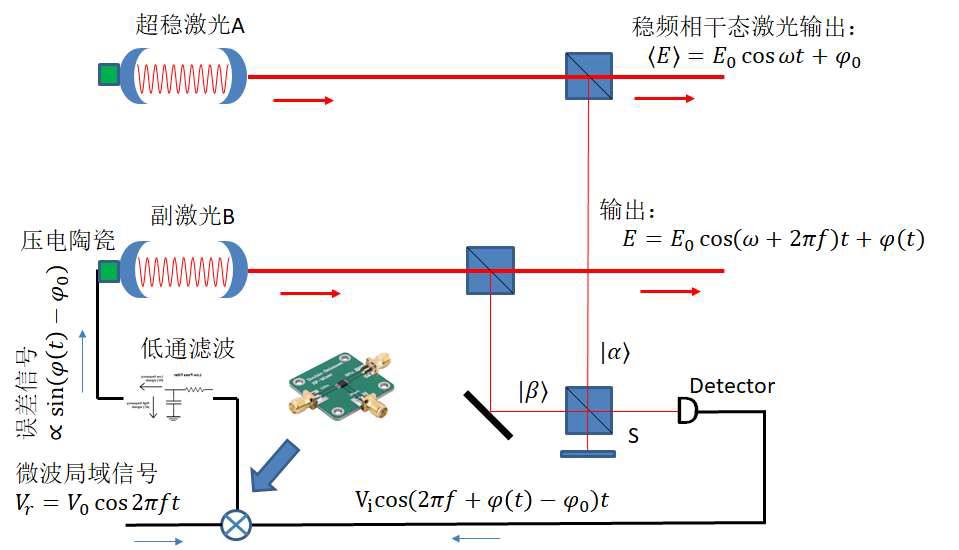
\includegraphics[width=0.6\textwidth]{phase-locking.png}
    \caption{A device for laser phase-locking}
    \label{fig:phase-locking}
\end{figure}

\paragraph{Laser phase-locking} \prettyref{fig:phase-locking} is a device for laser-phase locking. 
The detector is a ``continuous'' detector, which accumulates the photoelectrons generated in a time period and then releases the 
electrons, and therefore the detector is unable to detect details of the input light of which the characteristic time scale is 
below the time period. Suppose the characteristic time scale of the phase fluctuation is greater than the characteristic time scale of the detector, so the detector can be seen to reflect faithfully the input light without any coarse graining.
We use the following scheme to find the phase fluctuation: measure the  

\paragraph{Solution} We label the port corresponding to $\ket{\alpha}$ as $a^\dagger_1$, the port corresponding to $\ket{\beta}$ as $a^\dagger_2$, the port corresponding to the detector $b^\dagger_2$, and the port corresponding to $S$ as $b^\dagger_1$.
Then we have 
\[
    \pmqty{b^\dagger_1 \\ b^\dagger_2} = \frac{1}{\sqrt{2}} \pmqty{1 & -1 \\ 1 & 1} \pmqty{ a^\dagger_1 \\ a^\dagger_2 }.
\]
The expectation is 
\[
    \begin{aligned}
        \expval*{n_2} &= \mel*{\alpha, \beta}{b_2^\dagger b_2}{\alpha, \beta} \\
        &= \frac{1}{2} \mel*{\alpha, \beta}{ (a_1^\dagger + a_2^\dagger) (a_1 + a_2) }{\alpha, \beta} .
    \end{aligned}
\]
We choose a picture where $a_1^\dagger$ has no time evolution and the time evolution factor of $a_2^\dagger$ is $\ee^{\ii 2 \pi f t + \ii \varphi(t)}$, and therefore
\[
    \begin{aligned}
        \expval{n_2} &= \frac{1}{2} \mel*{\alpha, \beta}{ (a_1^\dagger(0) + a_2^\dagger(0) \ee^{\ii 2 \pi f t + \ii \varphi(t)}) (a_1(0) + a_2(0) \ee^{- \ii 2 \pi f t - \ii \varphi(t)}) }{\alpha, \beta} \\
        &= \frac{1}{2} \mel*{\alpha, \beta}{ (\alpha^* + \beta^* \ee^{\ii 2 \pi f t + \ii \varphi(t)}) (\alpha + \beta \ee^{- \ii 2 \pi f t - \ii \varphi(t)}) }{\alpha, \beta} .
    \end{aligned}
\]
Define the phase of $\alpha \beta^*$ as $\varphi_0$ and we have 
\begin{equation}
    \expval{n_2} = \frac{1}{2} (\abs*{\alpha}^2 + \abs*{\beta}^2 + 2 \abs*{\alpha} \abs*{\beta} \cos(2 \pi f t + \varphi(t) + \varphi_0)).
\end{equation}

Don't know what to do then ...

\paragraph{}

\paragraph{Measuring earth rotation with a Sagnac interferometer} In a Sagnac interferometer (see \prettyref{fig:sagnac-device}), input modes ${a}_{1}, {a}_{2}$ are mixed by a $50 \%$ - $50 \%$ beam splitter $S$, with its outputs follow ``time-reversal'' pathways of each other so as to be ``re-mixed'' by the same beam splitter $S$ into ${b}_{1}$ and ${b}_{2}$ modes.
(a) Express the linear transformation matrix that couples the input $a_{1}, a_{2}$ and output ${b}_{1}, {b}_{2}$ modes. Try to argue that in absence of rotation, the $2 \times 2$ transformation matrix ${S}$ is diagonal, i.e., when the $a_1$ port is seeded with a laser and $a_2$ port is left in vacuum state, then the $b_2$ output port is a ``dark port''.
(b) It turns out when the interferometer is placed in a rotating frame, such as on earth, the counter-propagating light paths around the loop with area $A$ can pick up a ``Sagnac'' phase,
\[
\varphi_{\text {sagnac }}=\frac{4 \pi \Omega \cdot A}{c \lambda}
\]
Here $\lambda$ is optical wavelength of the light. In presence of the Sagnac phase, derive the linear transformation matrix ${S}$ again.
(c) Consider $a_{1}$ mode is associated with pulsed laser input with duration $\tau=\SI{1}{ms}$.
The input states $\left|\psi_{\text{in}}\right\rangle=\ee^{\alpha a_{1}^{\dagger}-\alpha^{*} a_{1}}|V\rangle$ is a coherent state in the $a_{1}$ mode. For ${A}=\SI{1}{m^2}$, and let's consider the device is placed at the north pole. Suggest a detection scheme to measure the earth rotation rate (maybe quite difficult, if it is too difficult please allow yourself to be able to ``control'' the earth rotation). Assuming ideal detection, then how many photons are needed for the interferometer to measure earth rotation rate within $1 \%$ accuracy, using a single \SI{1}{ms} pulse?
(e) Provide a detailed argument that the $\Delta {n}_{2}$ shot noise for the ${n}_{2}=b_{2}^{\dagger} b_{2}$ measurement in this Sagnac interferometer is a result of vacuum fluctuation with $|V\rangle$ enters from the $a_{2}$ port to the $b_{2}$ port.
(f) Provide a plausible experimental arrangement to inject a ``squeezed vacuum'' into $a_{2}$ port, so as to improve the rotation measurement accuracy by a $\mathrm{e}^{\xi}$ factor.

\begin{figure}
    \centering
    

\tikzset{every picture/.style={line width=0.75pt}} %set default line width to 0.75pt        

\begin{tikzpicture}[x=0.75pt,y=0.75pt,yscale=-1,xscale=1]
%uncomment if require: \path (0,300); %set diagram left start at 0, and has height of 300

%Straight Lines [id:da8844772039784952] 
\draw    (420.79,85.53) -- (388.47,53.21) ;
%Straight Lines [id:da48446309467419546] 
\draw    (414.42,79.17) -- (423.32,79.17) ;
%Straight Lines [id:da726501602484074] 
\draw    (408.77,73.51) -- (417.67,73.51) ;
%Straight Lines [id:da7062627604246323] 
\draw    (402.4,67.15) -- (411.3,67.15) ;
%Straight Lines [id:da2274552840010844] 
\draw    (396.75,61.49) -- (405.65,61.49) ;
%Straight Lines [id:da5220705323464323] 
\draw    (391.09,55.83) -- (399.99,55.83) ;

%Straight Lines [id:da12364917794945707] 
\draw    (164.01,85.53) -- (196.32,53.21) ;
%Straight Lines [id:da4768126334948337] 
\draw    (170.37,79.17) -- (161.47,79.17) ;
%Straight Lines [id:da6808459516555925] 
\draw    (176.03,73.51) -- (167.13,73.51) ;
%Straight Lines [id:da09844706086771637] 
\draw    (182.39,67.15) -- (173.49,67.15) ;
%Straight Lines [id:da40837906298818916] 
\draw    (188.05,61.49) -- (179.15,61.49) ;
%Straight Lines [id:da35881747789081464] 
\draw    (193.7,55.83) -- (184.8,55.83) ;

%Straight Lines [id:da2687839088872306] 
\draw    (416.87,170.76) -- (384.55,203.08) ;
%Straight Lines [id:da6888141841763167] 
\draw    (410.51,177.13) -- (419.41,177.13) ;
%Straight Lines [id:da6720737631337188] 
\draw    (404.85,182.78) -- (413.75,182.78) ;
%Straight Lines [id:da7285323919972031] 
\draw    (398.49,189.15) -- (407.39,189.15) ;
%Straight Lines [id:da00960505985391591] 
\draw    (392.83,194.8) -- (401.73,194.8) ;
%Straight Lines [id:da7632489779797986] 
\draw    (387.18,200.46) -- (396.08,200.46) ;

%Shape: Square [id:dp020495620419631155] 
\draw   (201.78,163.22) -- (162,163.22) -- (162,203) -- (201.78,203) -- cycle ;
%Straight Lines [id:da14451433927098956] 
\draw    (201.78,203) -- (162,163.22) ;

%Straight Lines [id:da31388660860525963] 
\draw    (70.71,183.11) -- (197.89,183.11) ;
%Straight Lines [id:da33651403856752893] 
\draw    (197.89,183.11) -- (404.85,183.11) ;
%Straight Lines [id:da7165598417850927] 
\draw    (404.85,182.78) -- (404.85,69.37) ;
%Straight Lines [id:da9648860176265641] 
\draw    (180.16,69.37) -- (404.63,69.37) ;
%Straight Lines [id:da7876534442413605] 
\draw    (181.89,183.11) -- (181.89,69.7) ;
%Straight Lines [id:da11474982092647301] 
\draw    (181.89,262.22) -- (181.89,183.11) ;
%Straight Lines [id:da3039118324686805] 
\draw    (82.71,175.11) -- (111.71,175.11) ;
\draw [shift={(113.71,175.11)}, rotate = 180] [fill={rgb, 255:red, 0; green, 0; blue, 0 }  ][line width=0.08]  [draw opacity=0] (12,-3) -- (0,0) -- (12,3) -- cycle    ;
%Straight Lines [id:da20114092762893798] 
\draw    (109.71,192.11) -- (83.71,192.11) ;
\draw [shift={(81.71,192.11)}, rotate = 360] [fill={rgb, 255:red, 0; green, 0; blue, 0 }  ][line width=0.08]  [draw opacity=0] (12,-3) -- (0,0) -- (12,3) -- cycle    ;
%Straight Lines [id:da689329202115126] 
\draw    (172.71,260.22) -- (172.71,233.11) ;
\draw [shift={(172.71,231.11)}, rotate = 450] [fill={rgb, 255:red, 0; green, 0; blue, 0 }  ][line width=0.08]  [draw opacity=0] (12,-3) -- (0,0) -- (12,3) -- cycle    ;
%Straight Lines [id:da6858935984029761] 
\draw    (189.71,260.22) -- (189.71,233.11) ;
\draw [shift={(189.71,262.22)}, rotate = 270] [fill={rgb, 255:red, 0; green, 0; blue, 0 }  ][line width=0.08]  [draw opacity=0] (12,-3) -- (0,0) -- (12,3) -- cycle    ;

% Text Node
\draw (81,150.4) node [anchor=north west][inner sep=0.75pt]    {$a_{1}$};
% Text Node
\draw (83.71,195.51) node [anchor=north west][inner sep=0.75pt]    {$b_{1}$};
% Text Node
\draw (152,236.4) node [anchor=north west][inner sep=0.75pt]    {$a_{2}$};
% Text Node
\draw (191.71,236.51) node [anchor=north west][inner sep=0.75pt]    {$b_{2}$};


\end{tikzpicture}

    \caption{The Sagnac interferometer}
    \label{fig:sagnac-device}
\end{figure}

\paragraph{Solution} \begin{itemize}
    \item[(a)] The matrix of $S$ is 
    \[
        \frac{1}{\sqrt{2}} \pmqty{ 1 & -1 \\ 1 & 1 }.
    \]
    Its time reversal is 
    \[
        \frac{1}{\sqrt{2}} \pmqty{ 1 & 1 \\ -1 & 1 },
    \]
    and after being reflected by all the mirrors beam 1 is at the position of the output port 2 and beam 2 is at the position of the output port 1, so the transformation matrix for the two reflected beams can be obtained by swapping the columns of $S^\dagger$, so the final matrix of the whole system is 
    \begin{equation}
        S_\text{total} = \frac{1}{\sqrt{2}} \pmqty{ 1 & 1 \\ 1 & -1 } \cdot \frac{1}{\sqrt{2}} \pmqty{ 1 & -1 \\ 1 & 1 } = \pmqty{\dmat{1, -1}}.
    \end{equation} 
    The matrix is indeed diagonal, so port $b_2$ is a dark port without input in $a_2$ port.
    \item[(b)] Now the total matrix is 
    \begin{equation}
        \begin{aligned}
            S_\text{total}(\varphi) &= \frac{1}{\sqrt{2}} \pmqty{ 1 & 1 \\ 1 & -1 } \cdot \pmqty{\dmat{\ee^{\ii \varphi}, \ee^{- \ii \varphi}}} \cdot \frac{1}{\sqrt{2}} \pmqty{ 1 & -1 \\ 1 & 1 } \\
            &= \pmqty{ \cos \varphi & - \ii \sin \varphi \\ \ii \sin \varphi & - \cos \varphi },
        \end{aligned}
        \label{eq:sagnac-total-matrix}
    \end{equation} 
    where $\varphi$ is the Sagnac phase.
    \item[(c)] From
    \[
        \pmqty{b_1^\dagger \\ b_2^\dagger} = \pmqty{ \cos \varphi & - \ii \sin \varphi \\ \ii \sin \varphi & - \cos \varphi } \pmqty{a_1^\dagger \\ a_2^\dagger}
    \]
    we find 
    \begin{equation}
        \pmqty{a_1^\dagger \\ a_2^\dagger} = \pmqty{ \cos \varphi & - \ii \sin \varphi \\ \ii \sin \varphi & - \cos \varphi } \pmqty{b_1^\dagger \\ b_2^\dagger}.
    \end{equation}
    By substituting
    \[
        a_1^\dagger = \cos \varphi b_1^\dagger - \ii \sin \varphi b_2^\dagger
    \]
    into $\ket{\psi_\text{in}}$, we obtain 
    \begin{equation}
        \begin{aligned}
            \ket{\psi_\text{out}} &= \ee^{\alpha (\cos \varphi b_1^\dagger - \ii \sin \varphi b_2^\dagger) -\alpha^{*} (\cos \varphi b_1 + \ii \sin \varphi b_2)}|0\rangle \\
            &= \ket{\alpha \cos \varphi, - \ii \alpha \sin \varphi} .
        \end{aligned}
        \label{eq:out-state-sagnac}
    \end{equation}
    
    We need to measure $n_2$ with \eqref{eq:out-state-sagnac}.
    The expectation of $n_2$ is $\abs*{\alpha}^2 \sin^2 \varphi$, so the measure scheme may be measuring $n_2$ and calculating $\Omega$ using
    \begin{equation}
        \expval{n_2} = \abs*{\alpha}^2 \sin^2 \varphi , \quad \varphi = \frac{4 \pi \Omega \cdot A}{c \lambda}.
    \end{equation}

    From the properties of coherent states we also know that 
    \begin{equation}
        \Delta n_2 = \abs*{\alpha} \sin \varphi = \sqrt{\expval{n_2}}.
    \end{equation}
    Note that since $\varphi$ is small, we have 
    \[
        \expval*{n_2} \propto \varphi^2 \propto \Omega^2,
    \]
    so we have 
    \[
        \frac{2 \Delta \Omega}{\Omega} = \frac{\Delta n_2}{\expval*{n_2}} = \frac{1}{\sqrt{\expval{n_2}}},
    \]
    and therefore 
    \begin{equation}
        \expval{n_2} = \left( \frac{\Omega}{2 \Delta \Omega} \right)^2, \quad N_\text{in} = \abs*{\alpha}^2 = \left( \frac{c \lambda}{4 \pi \Omega A} \right)^2 \left( \frac{\Omega}{2 \Delta \Omega} \right)^2.
    \end{equation}
    Since the wavelength is not determined, the number of input photons cannot be determined.
    With the precision requirement $\Delta \Omega / \Omega = \SI{1}{\percent}$ we need at least to detect 2500 photons at the $b_2^\dagger$ port.
    \item[(e)] From (a) and (b), especially \eqref{eq:sagnac-total-matrix} and the fact that $\varphi \ll 1$, 
    we can view the whole system as an effective beam splitter with large transmission and small reflection.
    For this case % TODO: 
\end{itemize}

\paragraph{Discussion} Though we have an elegant relation between the required photon number at the \emph{output} port, 
experimentally people are more interested in the required photon number at the \emph{input} port or in other words what light source we should use.

\paragraph{}

\begin{figure}
    \centering
    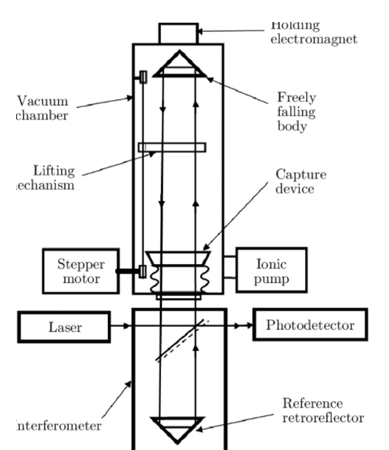
\includegraphics[width=0.6\textwidth]{free-fall.png}
    \caption{Measuring the position of a free-falling object}
    \label{fig:free-fall}
\end{figure}

\paragraph{Interferometric measurement of a free falling object} An optical circuit is built to measure the position of a free-falling object, shown in \prettyref{fig:free-fall}.
Analyze the accuracy of the equipment in terms of the wavelength and the power of the light beam.

\paragraph{Solution} The structure of the optical circuit of \prettyref{fig:free-fall} is quite like \prettyref{fig:sagnac-device}.
The main difference is that in \prettyref{fig:sagnac-device} a pulse may travel from one retroreflector to another over and over again.
The interferometer contains a cavity, and therefore a infinite sum is required to determine its behavior.
If the whole system is a two-port system, then no information about the distance between the freely falling body and the reference retroreflector can be passed out.
However, note that there is a second output port, so everything is fine here.

\paragraph{Discussion} Our calculation can be seen as the first order Doppler effect, 
where at each point we regard the cavity as a static one and the phase change is due to the shrinking cavity size.
Usually we do not need to take the whole Doppler effect into account since the free faller is always much slower than $c$.

What will really cause visible error is the light pressure to the freely falling body.
Generally speaking it is hard to amend this because the optical field has quantum fluctuation.

\paragraph{}

\begin{figure}
    

\tikzset{every picture/.style={line width=0.75pt}} %set default line width to 0.75pt        

\begin{tikzpicture}[x=0.75pt,y=0.75pt,yscale=-1,xscale=1]
%uncomment if require: \path (0,398); %set diagram left start at 0, and has height of 398

%Straight Lines [id:da8831059712635394] 
\draw    (141.89,101.11) -- (353.85,101.11) ;
%Shape: Square [id:dp7950538688502478] 
\draw   (157.16,85.84) -- (127,85.84) -- (127,116) -- (157.16,116) -- cycle ;
%Straight Lines [id:da6670768277096604] 
\draw    (157.16,116) -- (127,85.84) ;

%Straight Lines [id:da6385646046588365] 
\draw    (90.07,101.11) -- (141.89,101.11) ;
%Straight Lines [id:da38322783090861856] 
\draw    (141.89,101.11) -- (141.89,52.95) ;
%Straight Lines [id:da7853948154096531] 
\draw    (141.89,210.95) -- (141.89,101.11) ;
%Straight Lines [id:da015112676981859252] 
\draw    (369.79,117.53) -- (337.47,85.21) ;
%Straight Lines [id:da4746389539077047] 
\draw    (363.42,111.17) -- (372.32,111.17) ;
%Straight Lines [id:da46717262909625235] 
\draw    (357.77,105.51) -- (366.67,105.51) ;
%Straight Lines [id:da30525079380775666] 
\draw    (351.4,99.15) -- (360.3,99.15) ;
%Straight Lines [id:da44745460673622084] 
\draw    (345.75,93.49) -- (354.65,93.49) ;
%Straight Lines [id:da3815310434521484] 
\draw    (340.09,87.83) -- (348.99,87.83) ;

%Straight Lines [id:da6986475758735107] 
\draw    (124.92,193.76) -- (157.24,226.08) ;
%Straight Lines [id:da5720870142040946] 
\draw    (131.28,200.13) -- (122.38,200.13) ;
%Straight Lines [id:da2967706226479727] 
\draw    (136.94,205.78) -- (128.04,205.78) ;
%Straight Lines [id:da4042867119175786] 
\draw    (143.3,212.15) -- (134.4,212.15) ;
%Straight Lines [id:da9939960031496065] 
\draw    (148.96,217.8) -- (140.06,217.8) ;
%Straight Lines [id:da7251949462515492] 
\draw    (154.62,223.46) -- (145.72,223.46) ;

%Straight Lines [id:da6599104066857489] 
\draw    (143.3,212.15) -- (354.27,212.15) ;
%Straight Lines [id:da9897527492751317] 
\draw    (352.85,211.95) -- (352.85,101.11) ;
%Straight Lines [id:da5077844363253456] 
\draw    (352.89,280.95) -- (352.89,211.11) ;
%Straight Lines [id:da1391071580772758] 
\draw    (354.27,212.15) -- (438.71,212.15) ;
%Shape: Chord [id:dp7432077058406552] 
\draw   (368.14,281.09) .. controls (368.1,290.28) and (361.48,297.78) .. (353.19,297.93) .. controls (344.76,298.07) and (337.81,290.59) .. (337.64,281.21) -- cycle ;
%Shape: Square [id:dp6677275601543518] 
\draw   (368.16,196.84) -- (338,196.84) -- (338,227) -- (368.16,227) -- cycle ;
%Straight Lines [id:da3926416976932525] 
\draw    (368.16,227) -- (338,196.84) ;

%Shape: Chord [id:dp03366700888620455] 
\draw   (438.85,196.9) .. controls (448.04,196.93) and (455.54,203.55) .. (455.69,211.85) .. controls (455.83,220.27) and (448.35,227.23) .. (438.97,227.39) -- cycle ;
%Straight Lines [id:da4337905141355789] 
\draw    (352.89,317.84) -- (352.89,297.95) ;
%Straight Lines [id:da28024545163587966] 
\draw    (455.71,212.15) -- (487.71,212.15) ;
%Straight Lines [id:da09091747518635618] 
\draw    (352.89,317.84) -- (473.33,317.84) ;
%Straight Lines [id:da13890130222995545] 
\draw    (487.25,303.92) -- (487.71,212.15) ;
%Flowchart: Summing Junction [id:dp05799293146797191] 
\draw   (501.16,317.84) .. controls (501.16,310.15) and (494.93,303.92) .. (487.25,303.92) .. controls (479.56,303.92) and (473.33,310.15) .. (473.33,317.84) .. controls (473.33,325.52) and (479.56,331.75) .. (487.25,331.75) .. controls (494.93,331.75) and (501.16,325.52) .. (501.16,317.84) -- cycle ; \draw   (497.09,307.99) -- (477.4,327.68) ; \draw   (477.4,307.99) -- (497.09,327.68) ;
%Straight Lines [id:da15920849307038765] 
\draw    (501.16,317.84) -- (529.71,317.84) ;

% Text Node
\draw (89,76.4) node [anchor=north west][inner sep=0.75pt]    {$a_{1}^{\dagger }$};
% Text Node
\draw (146,43.4) node [anchor=north west][inner sep=0.75pt]    {$a_{2}^{\dagger }$};
% Text Node
\draw (217,76.4) node [anchor=north west][inner sep=0.75pt]    {$\mathrm{e}^{\mathrm{i} \varphi /2}$};
% Text Node
\draw (216,190.4) node [anchor=north west][inner sep=0.75pt]    {$\mathrm{e}^{-\mathrm{i} \varphi /2}$};
% Text Node
\draw (392,184.4) node [anchor=north west][inner sep=0.75pt]    {$b_{2}^{\dagger }$};
% Text Node
\draw (335,246.4) node [anchor=north west][inner sep=0.75pt]    {$b_{1}^{\dagger }$};
% Text Node
\draw (10,30.4) node [anchor=north west][inner sep=0.75pt]    {$\ket{\psi } =a_{1}^{\dagger } a_{2}^{\dagger }\ket{0}$};
% Text Node
\draw (511,294.4) node [anchor=north west][inner sep=0.75pt]    {$\langle :n_{1} n_{2} :\rangle $};


\end{tikzpicture}

    \caption{The M-Z interferometer}
    \label{fig:mz-interferometer}    
\end{figure}

\paragraph{Measuring a phase shift with a double-photon interferometer} A double-photon interferometer shown in \prettyref{fig:mz-interferometer} can be used to measure the phase shift $\varphi$.
Derive the output and the fluctuation.

\paragraph{Solution} The transformation matrix of \prettyref{fig:mz-interferometer} is 
\begin{equation}
    \begin{aligned}
        S &= \frac{1}{\sqrt{2}} \pmqty{ 1 & -1 \\ 1 & 1 } \cdot \pmqty{\dmat{\ee^{\ii \varphi / 2}, \ee^{- \ii \varphi / 2}}} \cdot \frac{1}{\sqrt{2}} \pmqty{ 1 & -1 \\ 1 & 1 } \\
        &= \pmqty{ \ii \sin \varphi / 2 & - \cos \varphi / 2 \\ \cos \varphi / 2 & - \ii \sin \varphi / 2 }.
    \end{aligned}
\end{equation}
We therefore have 
\begin{equation}
    \pmqty{a_1^\dagger \\ a_2^\dagger} = S^{-1} \pmqty{b_1^\dagger \\ b_2^\dagger} = \pmqty{ - \ii b_1^\dagger \sin \varphi / 2 + b_2^\dagger \cos \varphi / 2 \\ - b_1^\dagger \cos \varphi / 2 + \ii b_2^\dagger \sin \varphi / 2 }.
\end{equation}
The wave function of the optical field, therefore, is 
\begin{equation}
    \begin{aligned}
        \ket{\psi} &= a_1^\dagger a_2^\dagger \ket{0} = (- \ii b_1^\dagger \sin \varphi / 2 + b_2^\dagger \cos \varphi / 2) (- b_1^\dagger \cos \varphi / 2 + \ii b_2^\dagger \sin \varphi / 2) \ket{0} \\
        &= \frac{\ii}{\sqrt{2}} \sin \varphi \ket{2, 0} + \frac{\ii}{\sqrt{2}} \sin \varphi \ket{0, 2} - \cos \varphi \ket{1, 1}.
    \end{aligned}
\end{equation}

The expectation of $:n_1 n_2:$ is 
\begin{equation}
    \mel*{\psi}{b_1^\dagger b_2^\dagger b_2 b_1}{\psi} = \cos^2 \varphi 
\end{equation}
because the operators $b_1 b_2$ destroys $\ket{0, 2}$ and $\ket{2, 0}$, and we have 
\begin{equation}
    P(\text{result = $1$}) = \cos^2 \varphi, \quad P(\text{result = $2$}) = \sin^2 \varphi.
\end{equation}
The standard deviation is therefore given by
\[
    \begin{aligned}
        \Delta(: n_1 n_2 :)^2 &= P(\text{result = $1$}) (1 - \cos^2 \varphi)^2 + P(\text{result = $0$}) (0 - \cos^2 \varphi)^2 \\
        &= \cos^2 \varphi \sin^4 \varphi + \sin^2 \varphi \cos^4 \varphi \\
        &= \sin^2 \varphi \cos^2 \varphi,
    \end{aligned}
\]
or 
\begin{equation}
    \Delta(: n_1 n_2 :) = \sin \varphi \cos \varphi.
\end{equation}
With $N$ independent experiments (assuming $N$ is large), we have 
\[
    \sum \expval{: n_1 n_2 :} = N \cos^2 \varphi,
\]
and 
\[
    \Delta(\sum :n_1 n_2:) = \sqrt{N} \sin\varphi \cos \varphi.
\]
Therefore, we have 
\[
    \begin{aligned}
        \Delta\varphi &= \frac{\Delta(\sum :n_1 n_2:)}{\pdv*{\sum \expval{: n_1 n_2 :}}{\varphi}} \\
        &= \frac{\sqrt{N} \sin \varphi \cos \varphi}{N \times 2 \cos \varphi \sin \varphi} \\
        &= \frac{1}{2 \sqrt{N}},
    \end{aligned}
\]
so the fluctuation of $\varphi$ caused by the shot-noise error of the optical field is 
\begin{equation}
    \Delta\varphi = \frac{1}{2 \sqrt{N}}.
\end{equation}

\paragraph{Discussion} Note that in this problem we are actually analyzing a device beyond the standard quantum limit.
The two beam splitters and the two mirrors in \prettyref{fig:mz-interferometer} essentially form a single beam splitter, 
so the M-Z interferometer can be viewed as a nonlinear interferometer measuring the output of the Hong–Ou–Mandel effect:
The two input photons always go through the same path and feel the same phase shift, therefore rendering the measurement of 
the phase shift more effective.

\bibliographystyle{plain}
\bibliography{../optics/quantize,2} 

\end{document}